To evaluate our autoscaling system described above, we ran experiments
on two infrastructures: a homogeneous one (the DAS-4, a multi-cluster system
hosted by universities in The Netherlands~\cite{das4}) and a heterogeneous
one (the Amazon EC2 cloud~\cite{amazonEC2}). The goal of our experiments
was to evaluate and compare the three classes of customers by how well they fulfill 
the SLOs and by the amount of resources they allocate.

%In this section we conducted our experiments on a heterogeneous infrastructure like Amazon EC2~\cite{amazonEC2}, and on a homogeneous infrastructure like DAS-4 (the Distributed ASCI Supercomputer 4)~\cite{das4}. In our experiment campaign, we compared the degree of SLO enforcement and resource consumption for each provisioning algorithm implemented in ConPaaS. 

%DAS-4 is the Dutch Computational Infrastructure, a six-cluster wide-area distributed system designed with research purposes

\textbf{Testbed configuration:}  As a representative scenario, we deployed the MediaWiki application using ConPaaS on both infrastructures, and we ran the Wikibench tools with a 10\% sample of a real Wikipedia access trace for 24hours. 
%Consequently, our goal is to evaluate the behavior of the provisioning algorithms, when scaling out and back the number of VMs hosting PhP servers to guarantee several performance requirements, referred to as SLO.  Accordingly, some assumptions were made:
We configured the experiments as follows:

\begin{itemize}
\item  Response times from static requests were not analyzed due to its lightweight nature. 

\item The monitoring data was collected over a reporting period of 5 minutes.

\item We fixed a SLO of 700 milliseconds at the service's side.

\item We fixed a SLO penalty to half the price of a small instance per violation in any of the cloud infrastructures.

\item The algorithms used the same statistically-chosen performance threshold ranges. 

\item A minimum interval of 10 minutes has been established between scaling actions to avoid excessive oscillations. 
\end{itemize}


%To provide the Wikipedia services, an initial configuration was composed of 4 VMs, and 1 VM to host the Wikibench tools. The 4 VMs include a PhP service manager VM, a PhP agent VM, a web server and a http-proxy agent VM (both in the same VM), and finally a MySQL agent VM to store the English Wikipedia data, as explained in Section~\ref{wikipedia}.






\subsection{Heterogeneous Infrastructure}

\begin{table}
  {\scriptsize 
\begin{center}
    \begin{tabular}{  | c | c | c | c | c |}
    \hline
      \textbf{Name}  & \textbf{Configuration} & \textbf{Cost/hr} \\ \hline
   \textit{m1.small}   & 1-ECU~\footnote{One EC2 compute unit provides the equivalent CPU capacity of a 1.0-1.2 GHz 2007 Opteron or 2007 Xeon processor.}  -- 1.5Gb RAM&  0.06\$ \\ \hline
   \textit{m1.medium}   & 2-ECU -- 4Gb RAM&  0.12\$ \\ \hline
\textit{c1.medium} & 5-ECU -- 3Gb RAM& 0.145\$   \\ \hline
\textit{m1.large} & 4-ECU -- 8Gb RAM& 0.24\$   \\ \hline
 \end{tabular}
\end{center}
\vspace{-5mm}
\caption{EC2 instance type characteristics.}
\label{EC2instances}
}
\end{table}

\subsubsection{SLA fulfillment: low}

\begin{figure}
  \begin{center}
    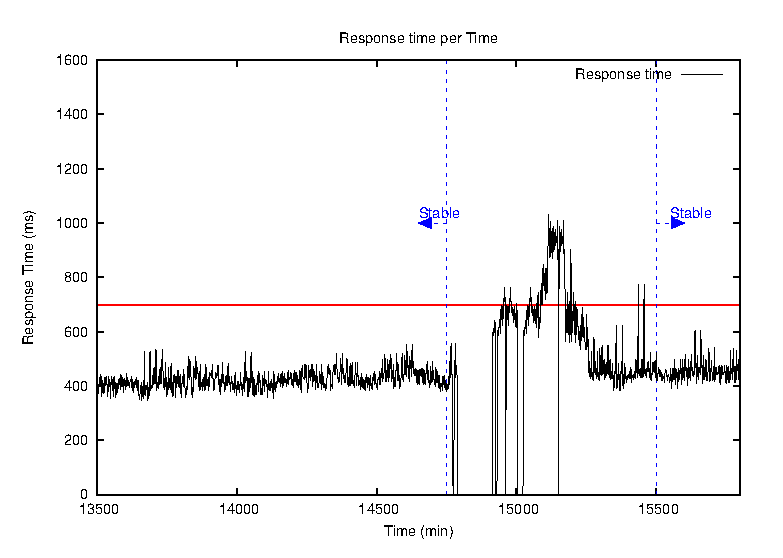
\includegraphics[width=.85\linewidth]{images/exps2011/low/ec2/proxyDataPoints_output_filtered.eps}
  \end{center}
\vspace{-5mm}
  \caption{EC2: Response time values for a bronze customer.}
  \label{lowResponseTime}
\end{figure}

\begin{figure}
  \begin{center}
    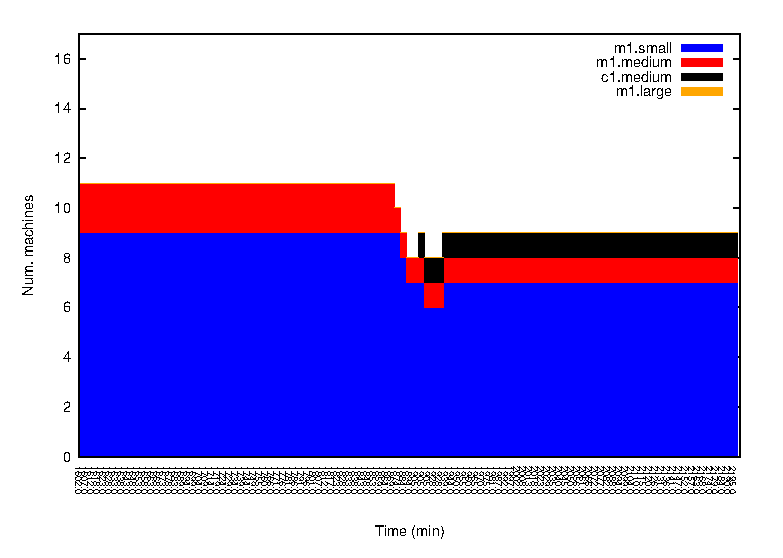
\includegraphics[width=.85\linewidth]{images/exps2011/low/ec2/inst_type_machines_filtered.eps}
  \end{center}
\vspace{-5mm}
  \caption{EC2: Cloud instances provisioned for a bronze customer.}
  \label{lowInstances}
\end{figure}

\begin{figure}
  \begin{center}
    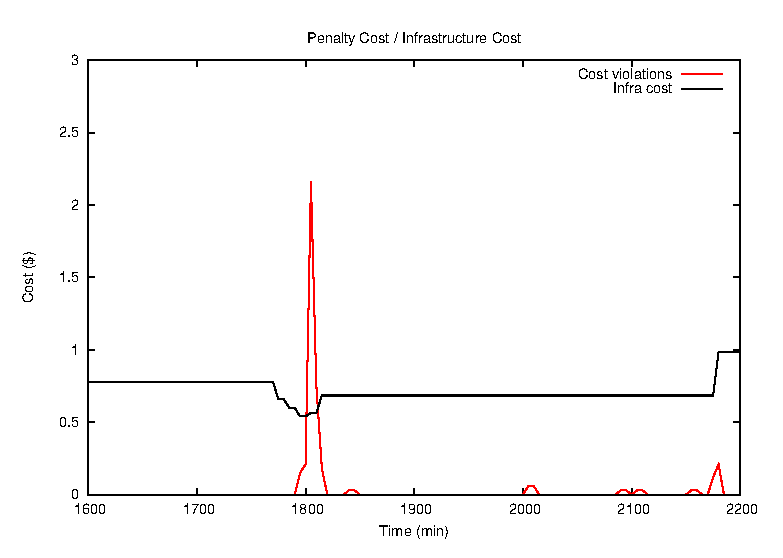
\includegraphics[width=.85\linewidth]{images/exps2011/low/ec2/penaltyVScost_filtered.eps}
  \end{center}
\vspace{-5mm}
  \caption{EC2: Infrastructure cost vs SLO violation penalty for a bronze customer.}
  \label{lowPenalty}
\end{figure}

\subsubsection{SLA fulfillment: medium}

\begin{figure}
  \begin{center}
    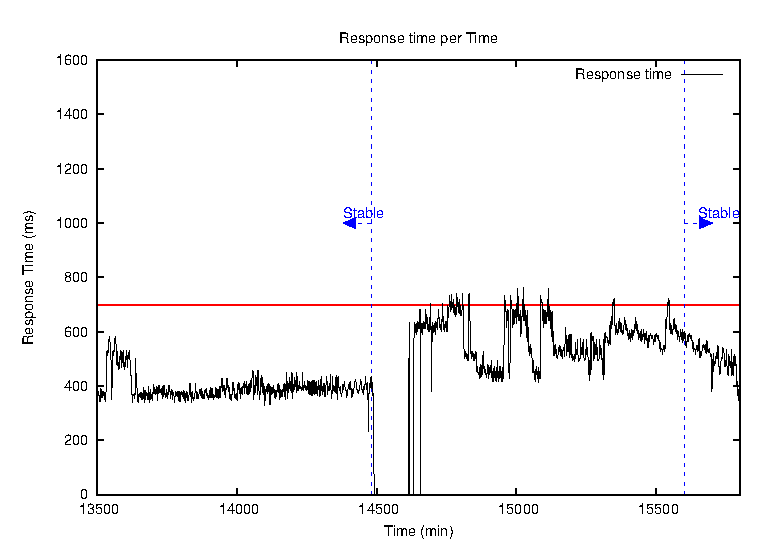
\includegraphics[width=.85\linewidth]{images/exps2011/medium/ec2/proxyDataPoints_output_filtered.eps}
  \end{center}
\vspace{-5mm}
  \caption{EC2: Response time values for a silver customer.}
  \label{zoomOutage}
\end{figure}

\begin{figure}
  \begin{center}
    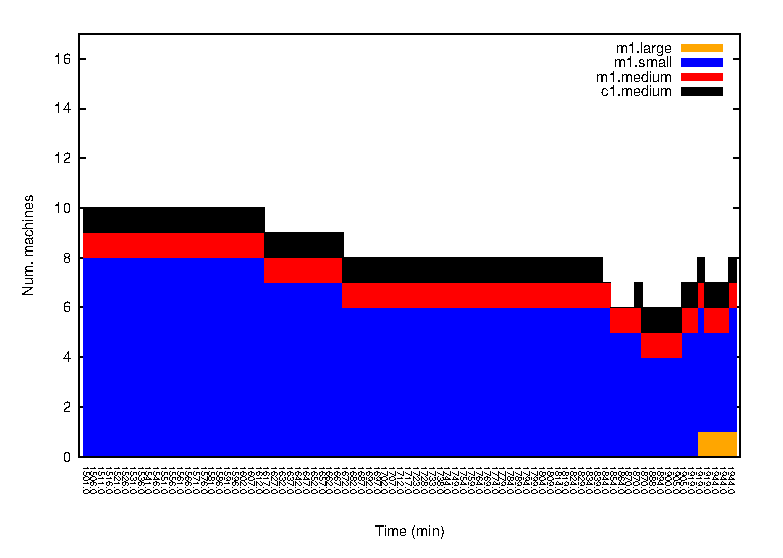
\includegraphics[width=.85\linewidth]{images/exps2011/medium/ec2/inst_type_machines_filtered.eps}
  \end{center}
\vspace{-5mm}
  \caption{EC2: Cloud instances provisioned for a silver customer.}
  \label{mediumInstances}
\end{figure}


\begin{figure}
  \begin{center}
    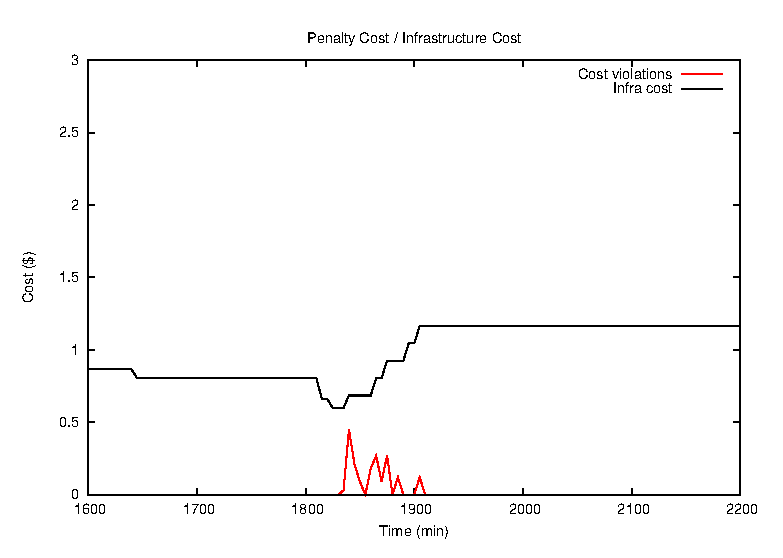
\includegraphics[width=.85\linewidth]{images/exps2011/medium/ec2/penaltyVScost_filtered.eps}
  \end{center}
\vspace{-5mm}
  \caption{EC2: Infrastructure cost vs SLO violation penalty for a silver customer.}
  \label{mediumPenalty}
\end{figure}

\subsubsection{SLA fulfillment: high}


\begin{figure}
  \begin{center}
    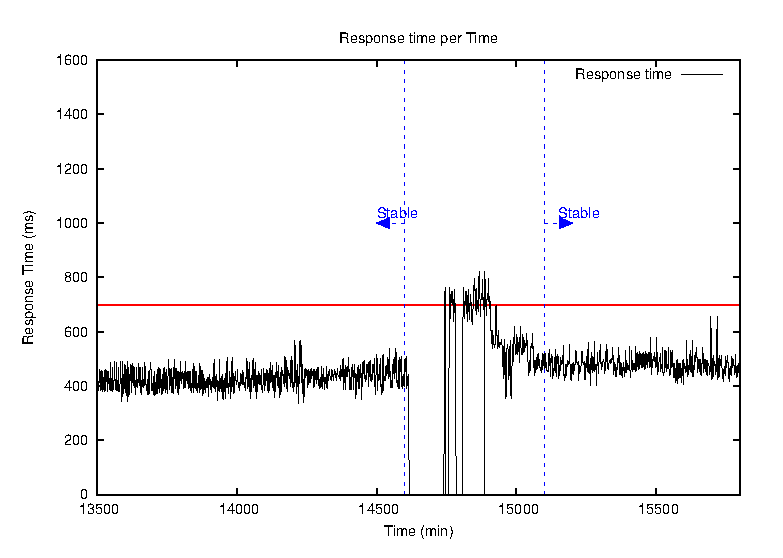
\includegraphics[width=.85\linewidth]{images/exps2011/high/ec2/proxyDataPoints_output_filtered.eps}
  \end{center}
\vspace{-5mm}
  \caption{EC2: Response time values for a gold customer.}
  \label{zoomOutage}
\end{figure}

\begin{figure}
  \begin{center}
    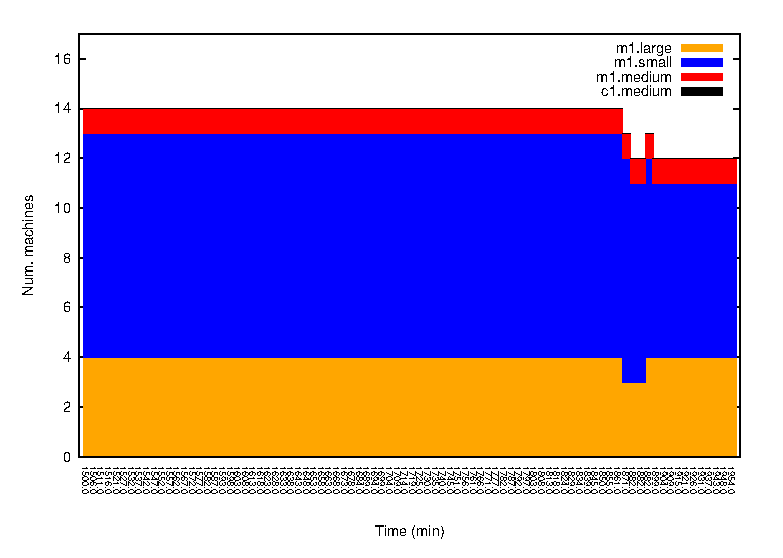
\includegraphics[width=.85\linewidth]{images/exps2011/high/ec2/inst_type_machines_filtered.eps}
  \end{center}
\vspace{-5mm}
  \caption{EC2: Cloud instances provisioned for a gold customer.}
  \label{resOutage}
\end{figure}

\begin{figure}
  \begin{center}
    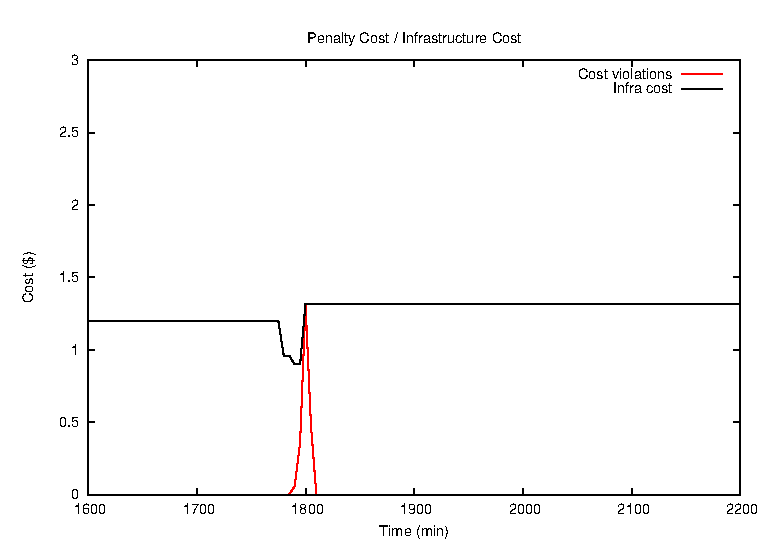
\includegraphics[width=.85\linewidth]{images/exps2011/high/ec2/penaltyVScost_filtered.eps}
  \end{center}
\vspace{-5mm}
  \caption{EC2: Infrastructure cost vs SLO violation penalty for a gold customer.}
  \label{highPenalty}
\end{figure}

\begin{table*}\label{summaryEC2}
  {\scriptsize 
\begin{center}
    \begin{tabular}{  | c | c | c | c | c |}
    \hline
         \textbf{Name}  & \textbf{SLO Violations} & \textbf{Decisions}  & \textbf{Cost}  & \textbf{Cost violations} \\ \hline
   \textit{Bronze}   &  1299 &  23 &  38.275\$ \$ & 38.97 \$ \\ \hline   
   \textit{Silver}  &  461 &  27 &  47,555\$ \$ &  13.83 \$ \\ \hline   
\textit{Gold} &   1007  &  19 &  59.4\$ \$ & 25.77 \$ \\ \hline   

 \end{tabular}
\end{center}
\vspace{-5mm}
\caption{Analysis of results on EC2}
\label{summaryEC2}
}
\end{table*}

%%% EXPERIMENTS DAS4 %%%%


\subsection{Homogeneous Infrastructure}

\begin{table}\label{DAS4instances}
  {\scriptsize 
\begin{center}
    \begin{tabular}{  | c | c | c | c | }
    \hline
       \textbf{Name}  & \textbf{Configuration} & \textbf{Cost/hr} \\ \hline
   \textit{small}   & 1-core 2.4Ghz -- 1Gb RAM&  0.05\$ \\ \hline
   \textit{medium}   & 4-core 2.4Ghz  -- 4Gb RAM&  0.23\$ \\ \hline
\textit{highcpu-medium} & 6-core 2.4Ghz -- 3Gb RAM& 0.28\$   \\ \hline
\textit{large} & 8-core 2.4Ghz  -- 8Gb RAM& 0.46\$   \\ \hline

 \end{tabular}
\end{center}
\vspace{-5mm}
\caption{DAS4 instance type characteristics.}
\label{DAS4instances}
}
\end{table}


\subsubsection{SLA fulfillment: low}

\begin{figure}
  \begin{center}
    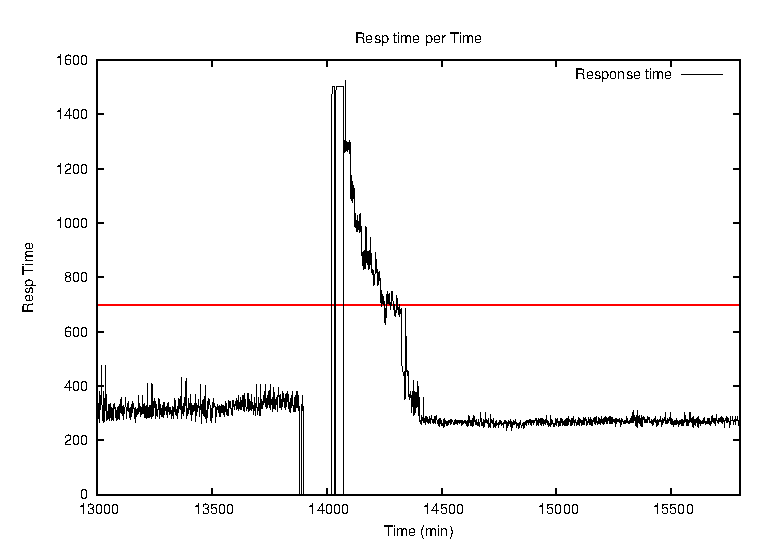
\includegraphics[width=.85\linewidth]{images/exps2011/low/das/proxyDataPoints_output_filtered.eps}
  \end{center}
\vspace{-5mm}
  \caption{DAS4: Response time values for a bronze customer.}
  \label{lowResponseTime}
\end{figure}



\begin{figure}
  \begin{center}
    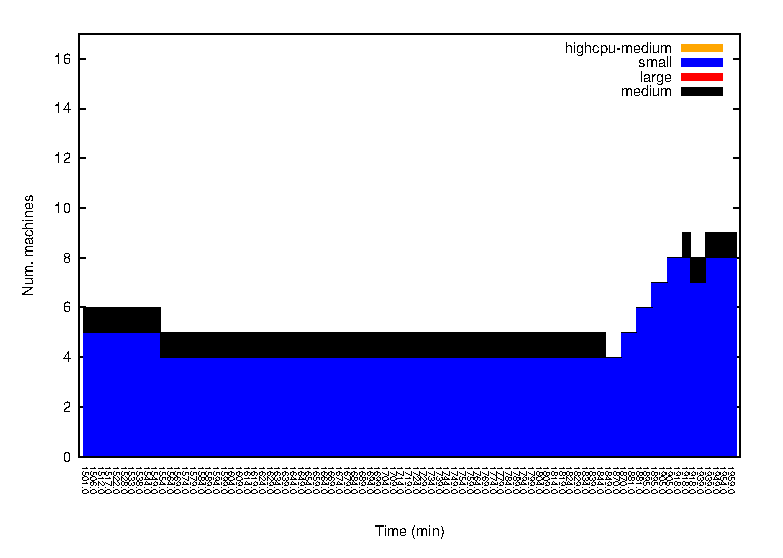
\includegraphics[width=.85\linewidth]{images/exps2011/low/das/inst_type_machines_filtered.eps}
  \end{center}
\vspace{-5mm}
  \caption{DAS4: Resource utilization during the outage for a bronze customer.}
  \label{resOutage}
\end{figure}


\begin{figure}
  \begin{center}
    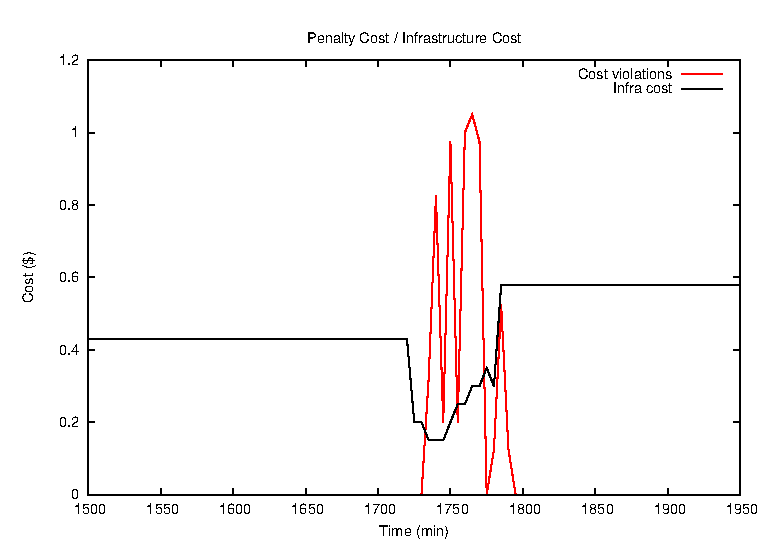
\includegraphics[width=.85\linewidth]{images/exps2011/low/das/penaltyVScost_filtered.eps}
  \end{center}
\vspace{-5mm}
  \caption{DAS4: Infrastructure cost vs SLO violation penalty for a bronze customer.}
  \label{lowPenalty}
\end{figure}

\subsubsection{SLA fulfillment: medium}

\begin{figure}
  \begin{center}
    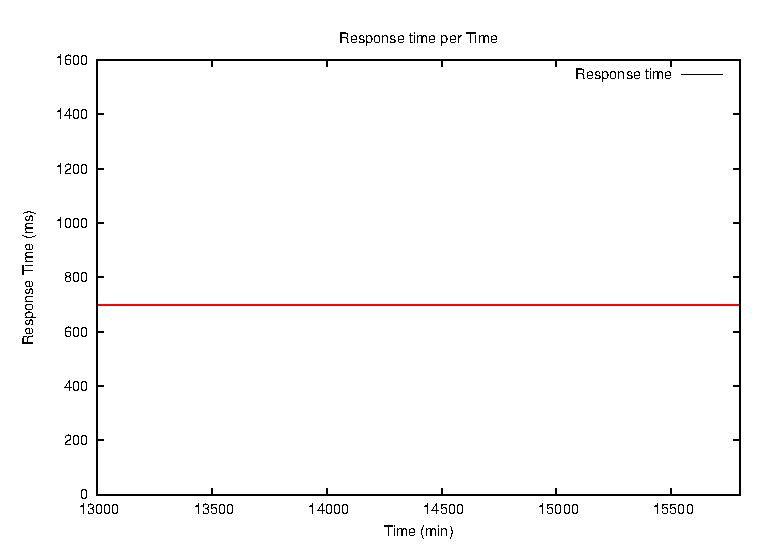
\includegraphics[width=.85\linewidth]{images/exps2011/medium/das/proxyDataPoints_output_filtered.eps}
  \end{center}
\vspace{-5mm}
  \caption{DAS4: Response time values for a silver customer.}
  \label{mediumResponseTime}
\end{figure}


\begin{figure}
  \begin{center}
    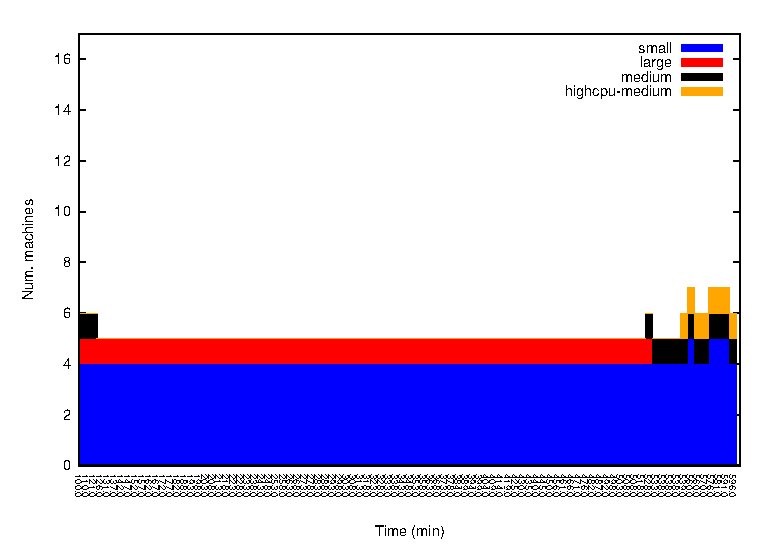
\includegraphics[width=.85\linewidth]{images/exps2011/medium/das/inst_type_machines_filtered.eps}
  \end{center}
\vspace{-5mm}
  \caption{DAS4: Cloud instances provisioned for a silver customer.}
  \label{mediumInstances}
\end{figure}



\begin{figure}
  \begin{center}
    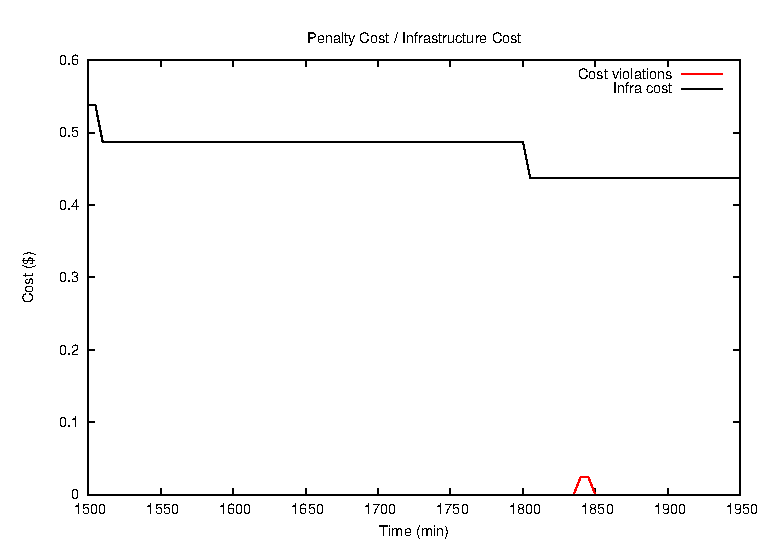
\includegraphics[width=.85\linewidth]{images/exps2011/medium/das/penaltyVScost_filtered.eps}
  \end{center}
\vspace{-5mm}
  \caption{DAS4: Infrastructure cost vs SLO violation penalty for a silver customer.}
  \label{mediumPenalty}
\end{figure}

\subsubsection{SLA fulfillment: high}

\begin{figure}
  \begin{center}
    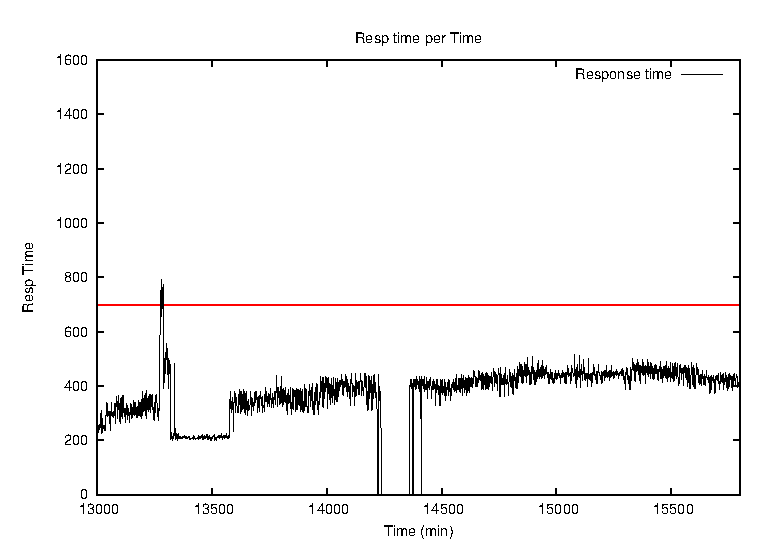
\includegraphics[width=.85\linewidth]{images/exps2011/high/das/proxyDataPoints_output_filtered.eps}
  \end{center}
\vspace{-5mm}
  \caption{DAS4: Response time values for a gold customer.}
  \label{highResponseTime}
\end{figure}


\begin{figure}
  \begin{center}
    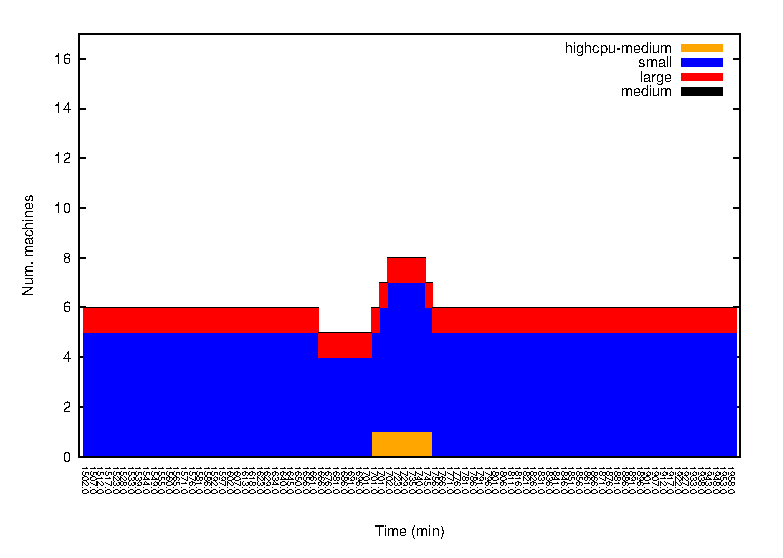
\includegraphics[width=.85\linewidth]{images/exps2011/high/das/inst_type_machines_filtered.eps}
  \end{center}
\vspace{-5mm}
  \caption{DAS4: Cloud instances provisioned for a gold customer.}
  \label{highInstances}
\end{figure}

\begin{figure}
  \begin{center}
    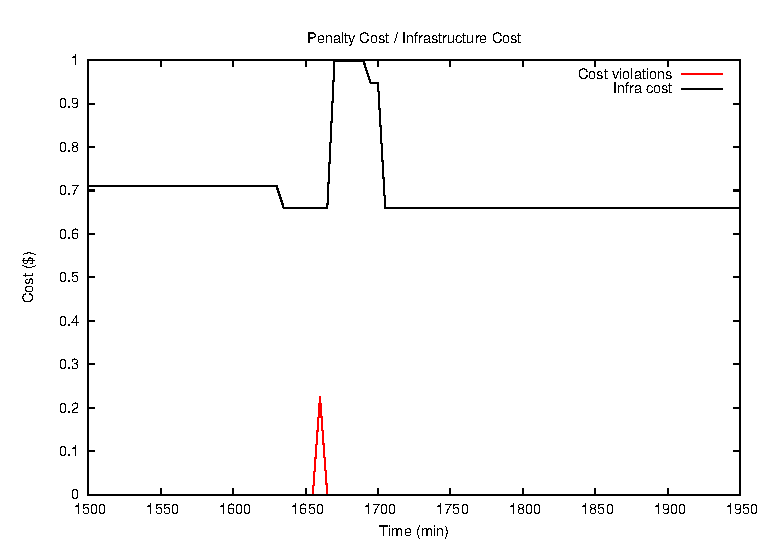
\includegraphics[width=.85\linewidth]{images/exps2011/high/das/penaltyVScost_filtered.eps}
  \end{center}
\vspace{-5mm}
  \caption{DAS4: Infrastructure cost vs SLO violation penalty for a gold customer.}
  \label{highPenalty}
\end{figure}

\begin{table*}
  {\scriptsize 
\begin{center}
    \begin{tabular}{  | c | c | c | c | c |}
    \hline
         \textbf{Name}  & \textbf{SLO Violations} & \textbf{Decisions}  & \textbf{Cost}  & \textbf{Cost violations} \\ \hline
   \textit{Bronze}   &  438 &  22 &  49.98\$ \$ & 13.14 \$ \\ \hline   
   \textit{Silver}  &  150 &  9 &  42.665\$ \$ &  4.5 \$ \\ \hline   
\textit{Gold} &  142 & 27 & 51.377\$ \$ & 3.81 \$ \\ \hline   

 \end{tabular}
\end{center}
\vspace{-5mm}
\caption{Analysis of results on DAS4}
\label{summaryDAS4}
}
\end{table*}
